\documentclass[12pt]{article}
	
%______________________PREAMBULO_________________________

%----------------------Paquetes--------------------------
\usepackage{amsmath,amssymb,amsfonts,latexsym,cancel} % Paquetes de símbolos adicionales.
\usepackage[spanish,es-tabla]{babel} % Idioma español
\usepackage[utf8]{inputenc} % Paquete que nos permite usar los acentos y otros símbolos, directamente del teclado.
\usepackage[T1]{fontenc} % Cambia el tipo de letra
\usepackage{times} % Tipo de letra Times New Roman
\usepackage{graphicx} % Paquete para el manejo de gráficos y figuras en el documento.
\usepackage{geometry} % Permite el manejo de los margenes
\usepackage{fancyhdr} % Permite colocar y manejar el encabezado
\usepackage[breaklinks,colorlinks=true,linkcolor=black,citecolor=blue, urlcolor=blue]{hyperref} % Crea hipervinculo entre secciones y el indice
\usepackage{pstricks}
%\usepackage{multicol}
%\usepackage{mathpazo} %fuente palatino
%\usepackage{xcolor}
%\usepackage[shortlabels]{enumitem}
%-------------Paquetes para el formato de las citas-------
%\usepackage[hyphens]{url}
%\usepackage{float}
%\usepackage{cite}
%\usepackage{wrapfig}

%-----------------------------ayuda de paquetes--------------------

\spanishdecimal{.}

%------------------------Margenes----------------------------

\newgeometry{bottom = 2.5 cm, top = 2.5 cm, left = 2 cm, right = 2 cm} % Modifica el margen {Abajo, Arriba, Izquierda, Derecha

%----------------------------Interlineado----------------------------------

%\doublespacing
%\onehalfspace
%\singlespace
%\spacing{1.5} % Permite personalisar a gusto
%\setlength{\parskip}{2cm} % Es el espacio entre parrafos

%-----------------------------Sangria---------------------------------------

\setlength{\parindent}{0 cm} % Manipula la sangria

%---------------------Portada------------------

%\title{
%\begin{figure}[h!]
		
%	\centering
%	
\includegraphics[width=\linewidth]{Nom_UAdeC_FCFM.png}  			
			
%\end{figure}
%\huge \textbf{LABORATORIO DE FISICA 3}\\\LARGE TITULO PRACTICA\\}
%\author{ \Large \textbf{Profesor:}\\
%\Large \textbf{Alumno:} Oscar Joel Castro Contreras}
%\date{\today}

%--------------Encabezado y pie de pagina--------------------

\pagestyle{fancy}%Coloca el encabezado en el documento
\lhead[]{Física 3}%Encabezado izquierda
\rhead[]{Oscar Joel Castro Contreras}%Encabesado derecha
%\chead[]{}%Encabesado central
\renewcommand{\headrulewidth}{0.08 pt}%Coloca linea al pie de pagina

%\lfoot[]{PI}%Pie de pagina izquerdo
%\rfoot[]{PD}%Pie de pagina derecho
\cfoot[]{\thepage}%Pie de pagina central
\renewcommand{\footrulewidth}{0.08 pt}%Coloca linea al pie de pagina

%-----------------------------------------------------------------------------

	\begin{document}
		
		\begin{titlepage}
		
			\centering
			{\bfseries
			\begin{figure}[h!]
				\centering
				
\includegraphics[width=\linewidth]{Nom_UAdeC_FCFM.png} 				
			\end{figure}
			\par}
			\vspace{2cm}
			{\scshape\LARGE FÍSICA 3 \par}
			\vspace{3cm}
			{\scshape\Huge \textbf{Tarea 2 - Ley de Gauss} \par}
			\vfill
			{\LARGE \textbf{Profesora:} Ricardo Pérez Martínez \par}
			\vspace{3cm}
			{\LARGE \textbf{Alumno:} Oscar Joel Castro Contreras \par}
			\vfill
			{\Large \today \par}
			\thispagestyle{empty}
			%\thispagestyle{fancy}
			
		\end{titlepage}
	
		\newpage
		
		\tableofcontents		
		
		\newpage
		
		\section*{Formulas:}\label{sec:Formulas}
			$$ k_e = 8.99 \times 10^9 \frac{Nm^2}{C^2} \quad \epsilon_0 = 8.8542 \times 10^{-12} \frac{C^2}{Nm^2} $$
			$$ \rho = \frac{Q}{V}, \quad \sigma = \frac{Q}{A}, \quad \lambda = \frac{Q}{L} $$
			$$ dq = \rho dV, \quad dq = \sigma dA, \quad dq = \lambda dL $$
			\begin{align}
				k_e &= \frac{1}{4\pi\epsilon_0} \nonumber \\
				\vec{F_e} &= q_0 \vec{E} \\
				\phi_E &= \oint EdA = \frac{q_{in}}{\epsilon_0}
			\end{align}

		\section{Problema 1:}\label{sec:Problema1}
			Sobre la superficie de una coraza esférica aislante de radio $ R $, está distribuida con
			uniformidad una carga negativa $ -Q $. Calcula la fuerza (magnitud y dirección) que
			ejerce la coraza sobre una carga puntual positiva $ q $ ubicada a una distancia:
			\begin{enumerate}
				\item[a)] $ r > R $ del centro de la coraza (fuera de la coraza).
						$$ \phi_E = \oint EdA = \frac{q_{in}}{\epsilon_0} $$
						$$ \phi_E = E \oint dA = E(4 \pi r^2) = \frac{-Q}{\epsilon_0} $$
						$$ E = \frac{-Q}{4 \pi r^2 \epsilon_0} = -k_e \frac{Q}{r^2} $$
						$$ \vec{F_e} = q_0 \vec{E} = -k_e \frac{Qq_0}{r^2} \hat{r} $$

				\item[b)] $ r < R $ del centro de la coraza (dentro de la coraza).
						$$ \phi_E = \oint EdA = \frac{q_{in}}{\epsilon_0} $$
						$$ \phi_E = E \oint dA = EA = 0 $$
						$$ E = 0 $$
			\end{enumerate}

		\section{Problema 2:}\label{sec:Problema2}
			Un conductor cílindrico de longitud infinita tiene un radio $ R $ y densidad superficial
			de carga uniforme $ \sigma $
			\begin{enumerate}
				\item[a)] En términos de $ \sigma $ y $ R $. ¿Cuál es la carga por unidad de longitud 
						$ \lambda $ para el cilindro?
						$$ dq = \sigma dA \quad dq = \lambda dl $$
						$$ q_{in} = \sigma 2 \pi R l \quad q_{in} = \lambda l  $$
						$$ \sigma = \frac{Q}{A} = \frac{Q}{\sigma 2 \pi R l} \quad \lambda = \sigma 2 \pi R $$
				\item[b)] En términos de $  \sigma $, ¿cuál es la magnitud del campo eléctrico producido 
						por el cilindro con carga a una distancia $ r > R $ de su eje?
						$$ \phi_E = \oint EdA = \frac{q_{in}}{\epsilon_0} $$
						$$ \phi_E = E \oint dA = E(2 \pi r l) = \frac{\sigma 2 \pi R l}{\epsilon_0} $$
						$$ E = \frac{\sigma R}{r \epsilon_0} $$
				\item[c)] Expresa el resultado del enciso b) en términos de $ \lambda $ y demuestra que el campo
						eléctrico fuera del cilindro es el mismo que si toda la carga estuviera sobre el eje.
						$$ \phi_E = \oint EdA = \frac{q_{in}}{\epsilon_0} $$
						$$ \phi_E = E \oint dA = E(2 \pi r l) = \frac{\lambda l}{\epsilon_0} $$
						$$ E = \frac{\lambda}{2 \pi r \epsilon_0} =  2k_e \frac{\lambda}{r} $$ \\
						$$ \phi_E = \oint EdA = \frac{q_{in}}{\epsilon_0} $$
						$$ \phi_E = E \oint dA =  E(2 \pi R l) = \frac{Q}{\epsilon_0} = \frac{Q}{2 \pi R l \epsilon_0} $$
						$$ E = 2 k_e \frac{Q}{Rl} $$
			\end{enumerate}
			Compara tu resultado c el que se obtuvo en clase para una línea infinita de carga. \\
			Se puede observar que la ecuación con sigma es distinta a la del lambda, pero cuando se 
			sustituye el valor de sigma y el de lambda las ecuaciones son iguales.

		\section{Problema 3:}\label{sec:Problema3}
			Una cubierta cilíndrica con un radio de $ 7.00cm $ y longitud de $ 240cm $ tiene una carga 
			con distribución uniforme sobre su superficie curva. La magnitud del campo eléctrico 
			un punto que está a $ 19.0cm $ radialmente hacia afuera de su eje (medido a partir 
			del punto medio de la cubierta) es de $ 36.0 \frac{kN}{C} $. Determine:
			$$ R = 7.00cm = 0.07m, \quad r = 19.0cm = 0.19m, \quad l = 240cm = 2.40m $$
			$$ E = 3.6 \frac{kN}{C} = 3.6 \times 10^4 \frac{N}{C} $$
			\begin{enumerate}
				\item[a)]	La carga neta sobre la cubierta.
						$$ dq = \sigma dA \Longrightarrow q_{in} = \sigma 2 \pi R l, \quad \sigma = \frac{Q}{A} = \frac{Q}{2 \pi R l} $$
						$$ \phi_E = \oint EdA = \frac{q_{in}}{\epsilon_0} $$
						$$ \phi_E = E \oint dA = E(2 \pi r l ) = \frac{\sigma 2 \pi R l}{\epsilon_0} $$
						$$ E = \frac{\sigma R}{r \epsilon_0} =  \left( \frac{Q}{2 \pi R l} \right) \frac{\sigma R}{r \epsilon_0} = \frac{Q}{2 \pi r l \epsilon_0} $$
						$$ E = 2 k_e \frac{Q}{rl} $$
						$$ Q = E\frac{rl}{2k_e} = \frac{(3.6 \times 10^4 \frac{N}{C})(0.19m)(2.40m)}{2(8.99 \times 10^9 \frac{Nm^2}{C^2})} $$
						$$ Q = 9.13 \times 10^{-7} C $$
				\item[b)] El campo eléctrico que existe en un punto a $ 4.00cm $ del eje, medido 
						radialmente hacia afuera del punto medio de la cubierta. \\
						La superficie gaussiana está dentro de la cubierta cilíndrica, la superficie 
						gaussiana no encierra ninguna carga por lo:
						$$ E = 0 $$
			\end{enumerate}

		\section{Problema 4:}\label{sec:Problema4}
			Un alambre largo y recto, rodeado por un cilindro de metal hueco cuyo eje coincide 
			con el suyo, tiene una carga por unidad de longitud $ L $, y el cilindro una carga por 
			unidad de longitud $ 2L $. Con esta información, utilice la ley de Gauss para determinar:  
			$$ q_a = \lambda L, \quad q_c = 2 \lambda L $$
			\begin{enumerate}
				\item[a)]	La carga por unidad de longitud en las superficies interna y externa del cilindro.
						$$ \lambda = \frac{q_c}{2l} $$ 
						$$ \phi_E = \oint EdA = \frac{q_{in}}{\epsilon_0} $$
						$$ \phi_E = E \oint dA = E(2 \pi R L)= \frac{\lambda L}{\epsilon_0} $$
						$$ E = \frac{\lambda}{2 \pi R \epsilon_0} = 2 k_e \frac{\lambda}{R} = 2 k_e \frac{1}{R} \left( \frac{q_c}{2l} \right) $$
						$$ E = k_e \frac{q_c}{LR} $$
						$$ q_c = \frac{ELR}{k_e} $$
				\item[b)] El campo eléctrico exterior al cilindro, a una distancia $ r $ de su eje.
						$$ q_t = q_a + q_c = \lambda L + 2 \lambda L = 3 \lambda L, \quad \lambda = \frac{q_t}{3L} $$
						$$ \phi_E = \oint EdA = \frac{q_{in}}{\epsilon_0} $$
						$$ \phi_E = E \oint dA = E(2 \pi r L)= \frac{3 \lambda L}{\epsilon_0} $$
						$$ E = \frac{3 \lambda}{2 \pi r \epsilon_0} = 2 k_e \frac{3\lambda}{r} = 6 k_e \frac{\lambda}{r} $$
						$$ E = 6 k_e \frac{1}{r} \left( \frac{q_t}{3L} \right) = 2 k_e \frac{q_t}{rL}$$
			\end{enumerate}

		\section{Problema 5:}\label{sec:Problema5}
			Una delgada placa conductora y cuadrada de $ 50.0cm $ de lado se encuentra sobre el 
			plano $ xy $. Se deposita una carga total de $ 4 \times 10^{-8} C $ sobre la placa. Determine: 
			$$ l = 50.0cm = 0.05m, \quad Q = 4 \times 10^{-8} C  $$
			\begin{enumerate}
				\item[a)]	La densidad de carga sobre la placa.
						$$ dq = \sigma dA \Longrightarrow q_{in} = \sigma l^2, \quad \sigma = \frac{Q}{A} = \frac{Q}{l^2} $$
				\item[b)]	El campo eléctrico justo por encima de la placa.
						$$ \phi_E = \oint EdA = \frac{q_{in}}{\epsilon_0} $$
						$$ \phi_E = E \oint dA = E(l^2)= \frac{Q}{\epsilon_0} $$
						$$ E = \frac{Q}{l^2 \epsilon_0} $$
						$$ E = \frac{Q}{l^2 \epsilon_0} = \frac{(4 \times 10^-{8} C)}{(0.05^2(8.8542 \times 10^{12} \frac{C^2}{Nm^2})} $$ 
						$$ E = 1.81 \times 10^{-18} \frac{N}{C} $$
				\item[c)] El campo eléctrico justo por debajo de la misma. La densidad de carga es uniforme. \\
						Como la densidad de carga es uniforme en la placa, la parte de de abajo de la placa tiene el mismo campo eléctrico que la parte de arriba.
			\end{enumerate}

		\section{Problema 6:}\label{sec:Problema6}
			Un cilindro largo de radio $ R $ con una densidad de carga que es proporcional a la 
			distancia a partir de su eje: $ \rho = kr $, donde $ k $ es una constante y $ r \in (0,R) $. Encuentra 
			el campo eléctrico dentro del cilindro, es decir, para puntos $ 0 < r < R $.
			$$ \rho = kr $$
			$$ dq = \rho dV \Longrightarrow q_{in} = \rho \pi r^2 l $$
			$$ \phi_E = \oint EdA = \frac{q_{in}}{\epsilon_0} $$
			$$ \phi_E = E \oint dA = E(2 \pi r l) = \frac{\rho \pi r^2 l }{\epsilon_0} $$
			$$ E = \frac{\rho r}{2 \epsilon_0} = \frac{(kr) r}{2 \epsilon_0} = \frac{k r^2}{2 \epsilon_0} $$

		\section{Problema 7:}\label{sec:Problema7}
			Un cascarón esférico con espesor, de radio interno $ a $ y radio externo $ b $, tiene una 
			densidad de carga $ \rho = \frac{k}{r^2} $ en la región $ a \leq r \leq b $. Encuentra el campo eléctrico en 
			las tres regiones: 
			\begin{enumerate}
				\item[I)]	 $ r < a $
						 $$ \phi_E = \oint EdA = \frac{q_{in}}{\epsilon_0} $$
						 $$ \phi_E = E \oint dA = EA = 0 $$ 
						 $$ E = 0 $$
				\item[II)] $ a < r < b $
						 $$ V = \frac{4 \pi b^3}{3} - \frac{4 \pi a^3}{3} = \frac{4 \pi}{3}(b^3-a^3) $$
						 $$ dq = \rho dV \Longrightarrow q_{in} = \rho \frac{4 \pi}{3}(b^3-a^3), \quad \rho = \frac{k}{r^2} $$
						 $$ \phi_E = \oint EdA = \frac{q_{in}}{\epsilon_0} $$
						 $$ \phi_E = E \oint dA = E(4 \pi r^2) = \rho \frac{4 \pi}{3 \epsilon_0}(b^3-a^3) $$ 
						 $$ E = \frac{\rho(b^3-a^3)}{3 r^2 \epsilon_0} = \left( \frac{k}{r^2} \right) \frac{b^3-a^3}{3 r^2 \epsilon_0} $$
						 $$ E = \frac{k(b^3-a^3)}{3 r^4 \epsilon_0} $$
				\item[III)]$ r > b $..
						 $$ \phi_E = \oint EdA = \frac{q_{in}}{\epsilon_0} $$
						 $$ \phi_E = E \oint dA = E(4 \pi r^2) = \rho \frac{Q}{\epsilon_0} $$
						 $$ E = \frac{Q}{4 \pi r^2 \epsilon_0} = k_e \frac{Q}{r^2} $$
			\end{enumerate}
			Realiza una gráfica del campo eléctrico. En función de $ r $.

			\begin{center}
				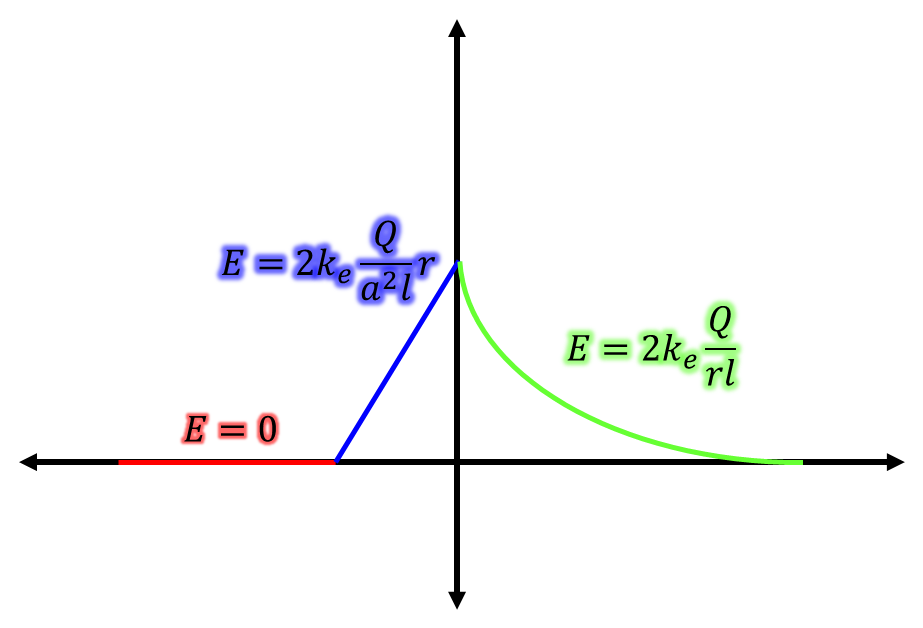
\includegraphics[width=.9\linewidth]{Fig 1.png}
			\end{center}

		\section{Problema 8:}\label{sec:Problema8}
			Un cable coaxial largo tiene una densidad de carga volumétrica uniforme en el cilindro 
			interno de radio $ a $ y una densidad superficial de carga uniforme en el cascarón
			cilíndrico externo de radio $ b $, $ b > a $. Esta carga superficial es negativa y con 
			magnitud tal que todo el cable coaxial es eléctricamente neutro. Encuentra el campo
			eléctrico en las tres regiones: 
			\begin{enumerate}
				\item[I)]	 Dentro del cilindro interno $ (r < a) $.
						 $$ dq = \rho dV \Longrightarrow q_{in} = \rho \pi r^2 l, \quad \rho = \frac{Q}{V} = \frac{Q}{\pi a^2 l} $$
						 $$ \phi_E = \oint EdA = \frac{q_{in}}{\epsilon_0} $$
						 $$ \phi_E = E \oint dA = E(2 \pi r l) = \frac{\rho \pi r^2 l}{\epsilon_0} $$ 
						 $$ E = \frac{\rho r}{2 \epsilon_0} = \left( \frac{Q}{\pi a^2 l} \right) \frac{r}{2 \epsilon_0} $$
						 $$ E = \frac{Qr}{2 \pi a^2 l \epsilon_0} = 2 k_e \frac{Q}{a^2 l} r $$
				\item[II)] Entre los cilindros $ (a < r < b) $.
						 $$ \phi_E = \oint EdA = \frac{q_{in}}{\epsilon_0} $$
						 $$ \phi_E = E \oint dA = E(2 \pi r l) = \frac{Q}{\epsilon_0} $$
						 $$ E = \frac{Q}{2 \pi r l \epsilon_0} = 2k_e \frac{Q}{rl} $$
				\item[III)]fuera del cable coaxial $ (r > b) $.
						  $$ q_{in} = Q - Q = 0 $$
						  $$ \phi_E = \oint EdA = \frac{q_{in}}{\epsilon_0} $$
						  $$ \phi_E = E \oint dA = EA = 0 $$
						  $$ E = 0 $$
			\end{enumerate}

	\end{document}